\def\layersep{1.5cm}
\begin{scope}[shorten >=1pt,->,draw=black!50, node distance=\layersep, scale=0.6, every node/.append style={transform shape},transform shape, local bounding box=ffnn]
  \tikzstyle{every pin edge}=[<-,shorten <=1pt]
  \tikzstyle{neuron}=[circle,fill=black!50,minimum size=17pt,inner sep=0pt]
  \tikzstyle{input neuron}=[neuron, fill=green!80];
  \tikzstyle{output neuron}=[neuron, fill=red!80];
  \tikzstyle{hidden neuron}=[neuron, fill=blue!80];
  \tikzstyle{annot} = [text width=4em, text centered]

  % Draw the input layer nodes
  \foreach \name / \y in {1,...,4}
  % This is the same as writing \foreach \name / \y in {1/1,2/2,3/3,4/4}
  % \node[input neuron, pin=left:Input \#\y] (I-\name) at (0,-\y) {};
  \node[input neuron, pin=left:{}] (I-\name) at (0,-\y) {};


  % Draw the hidden layer nodes
  \foreach \name / \y in {1,...,4}
  \path[yshift=0.0cm] node[hidden neuron] (H-\name) at (\layersep,-\y cm) {};

  % Draw the output layer node
  \foreach \name / \y in {1,...,4}
  \node[output neuron,pin={[pin edge={->}]right:{}}] (O-\name) at (2*\layersep, -\y cm) {};

  % Connect every node in the input layer with every node in the
  % hidden layer.
  \foreach \source in {1,...,4}
  \foreach \dest in {1,...,4}
  \draw[-{Stealth[scale=0.5]}] (I-\source) edge (H-\dest);

  % Connect every node in the hidden layer with the output layer
  \foreach \source in {1,...,4}
  \foreach \dest in {1,...,4}
  \draw[-{Stealth[scale=0.5]}] (H-\source) edge (O-\dest);

  % \foreach \source in {1,...,4}
  % \path (H-\source) edge (O);

  % Annotate the layers
  % \node[annot,above of=H-1, node distance=1cm] (hl) {Hidden layer};
  % \node[annot,left of=hl] {Input layer};
  % \node[annot,right of=hl] {Output layer};
  \node[inner sep=0pt, left= 0.2cm of ffnn] (latentz) {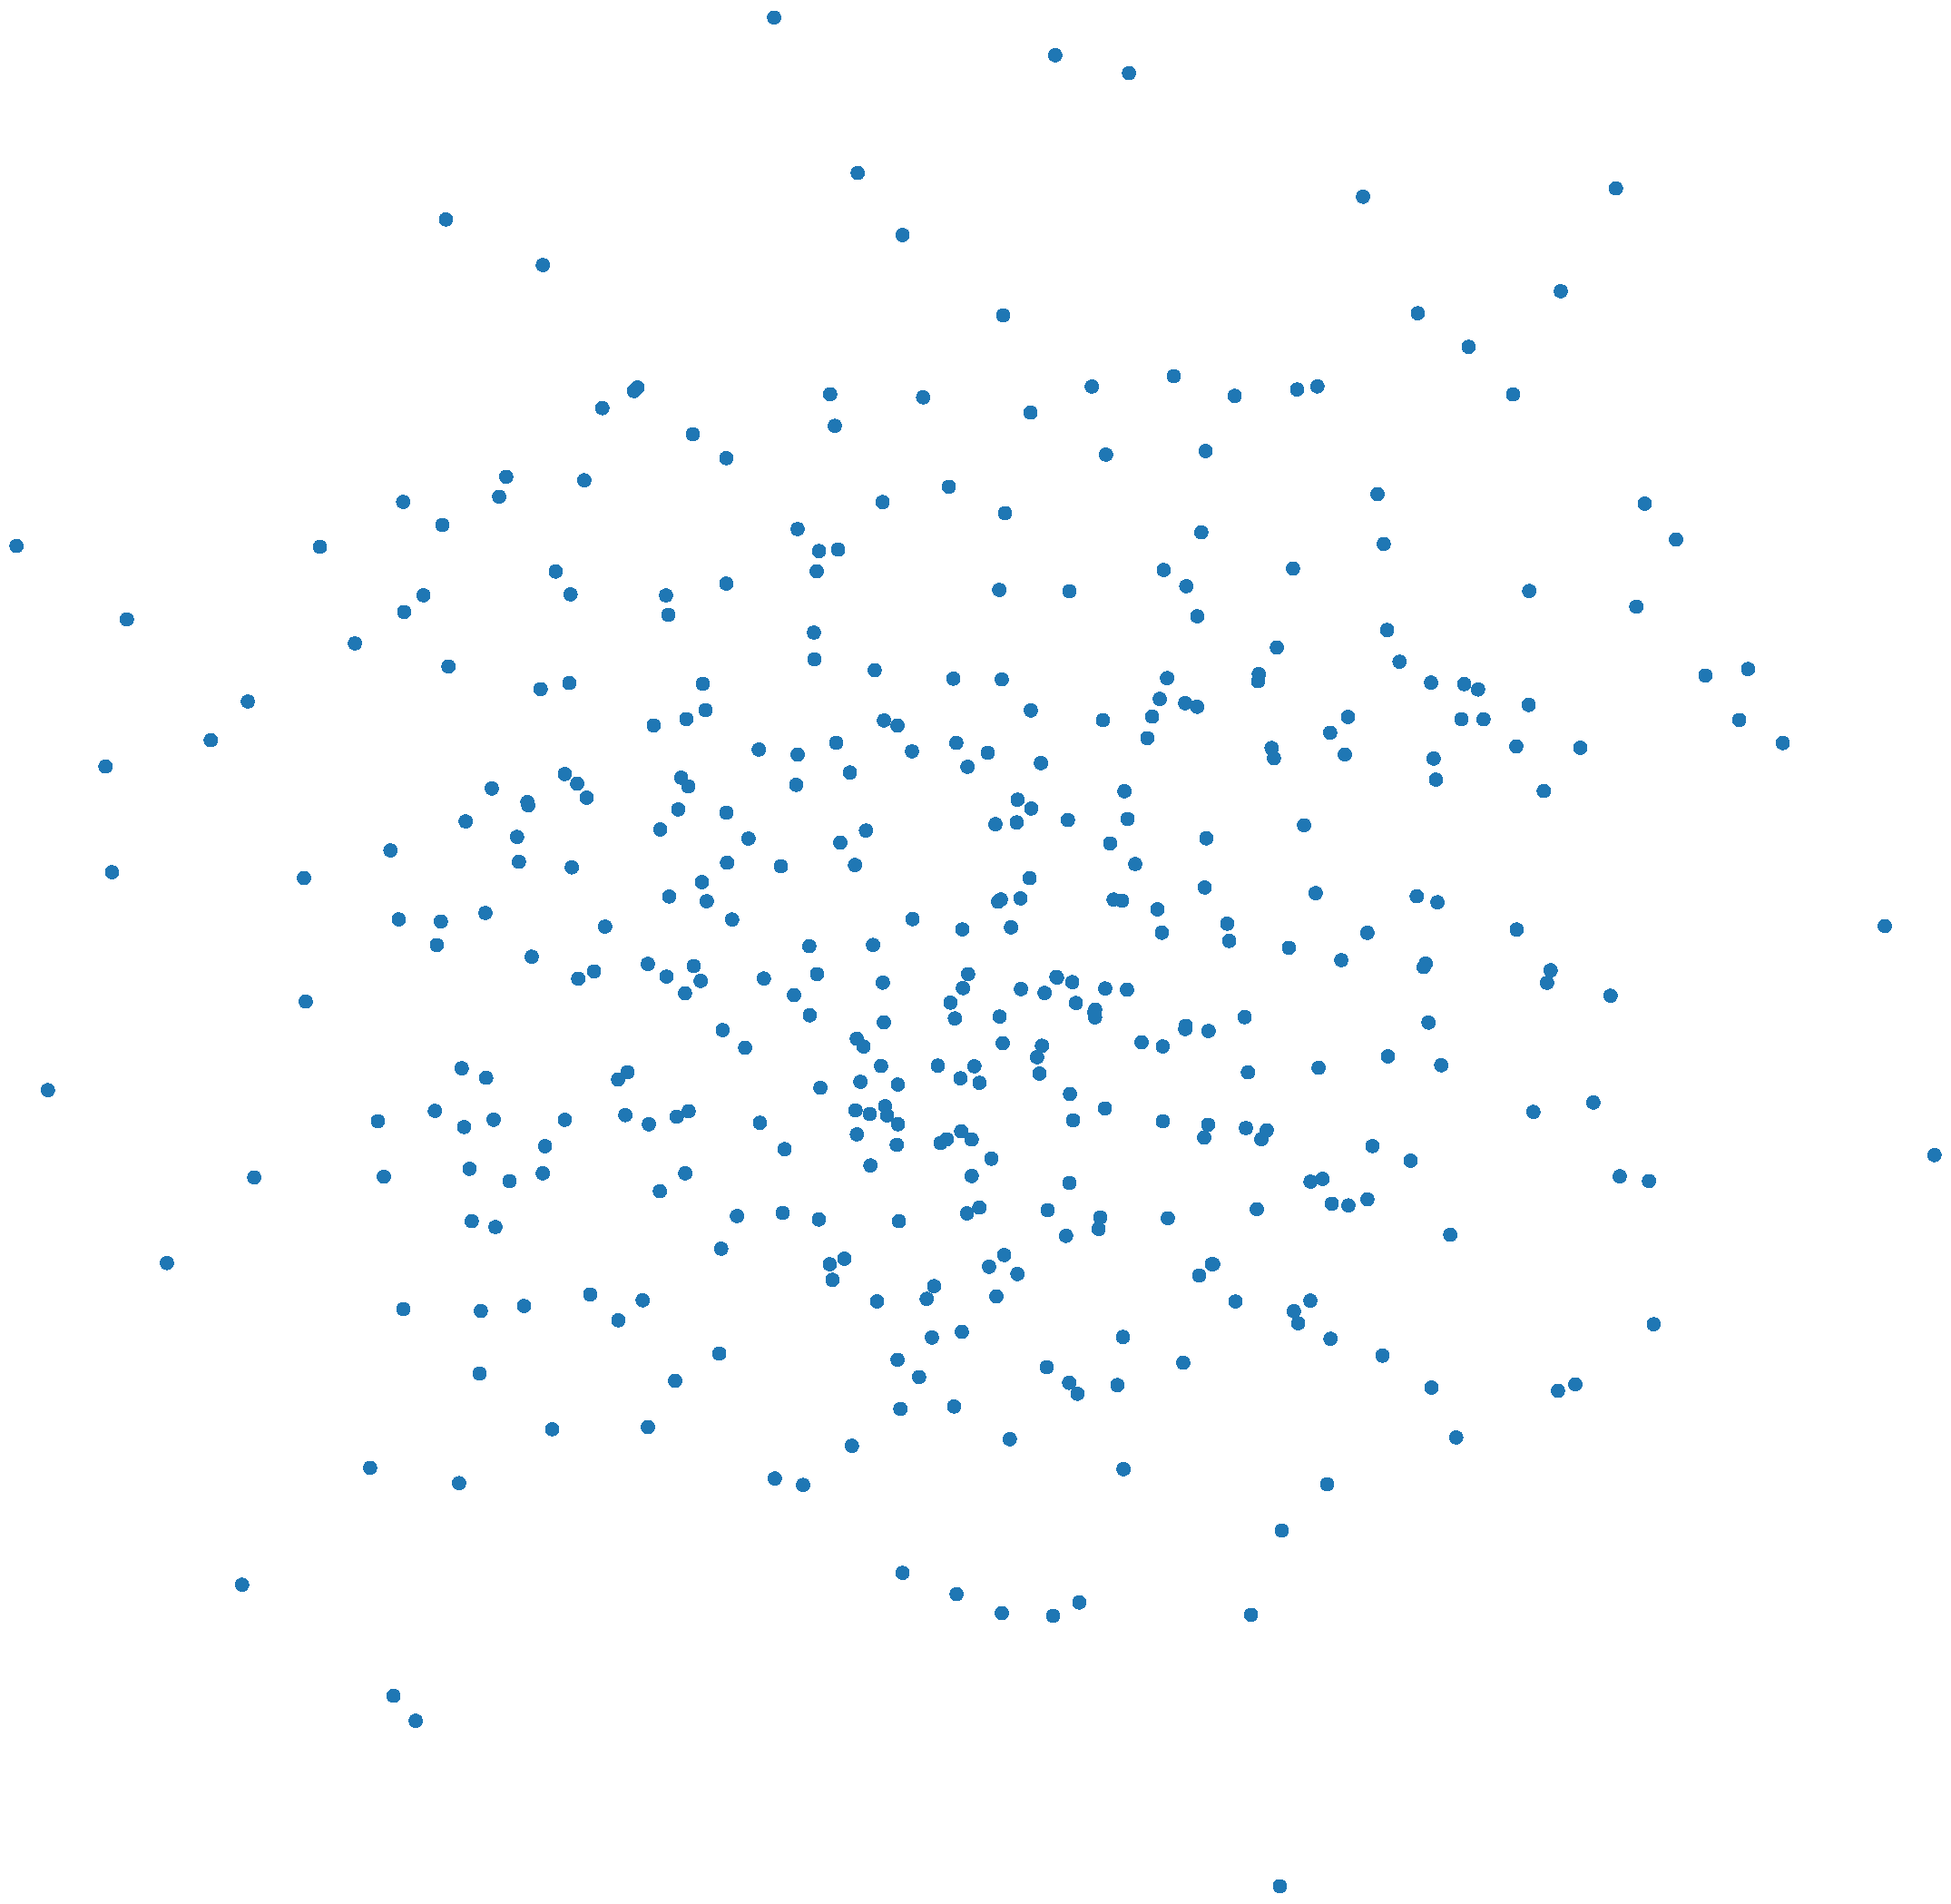
\includegraphics[width=.3\textwidth]{images/moon/zdist-crop.pdf}};
  \node[inner sep=0pt, right= 0.2cm of ffnn] (latentx) {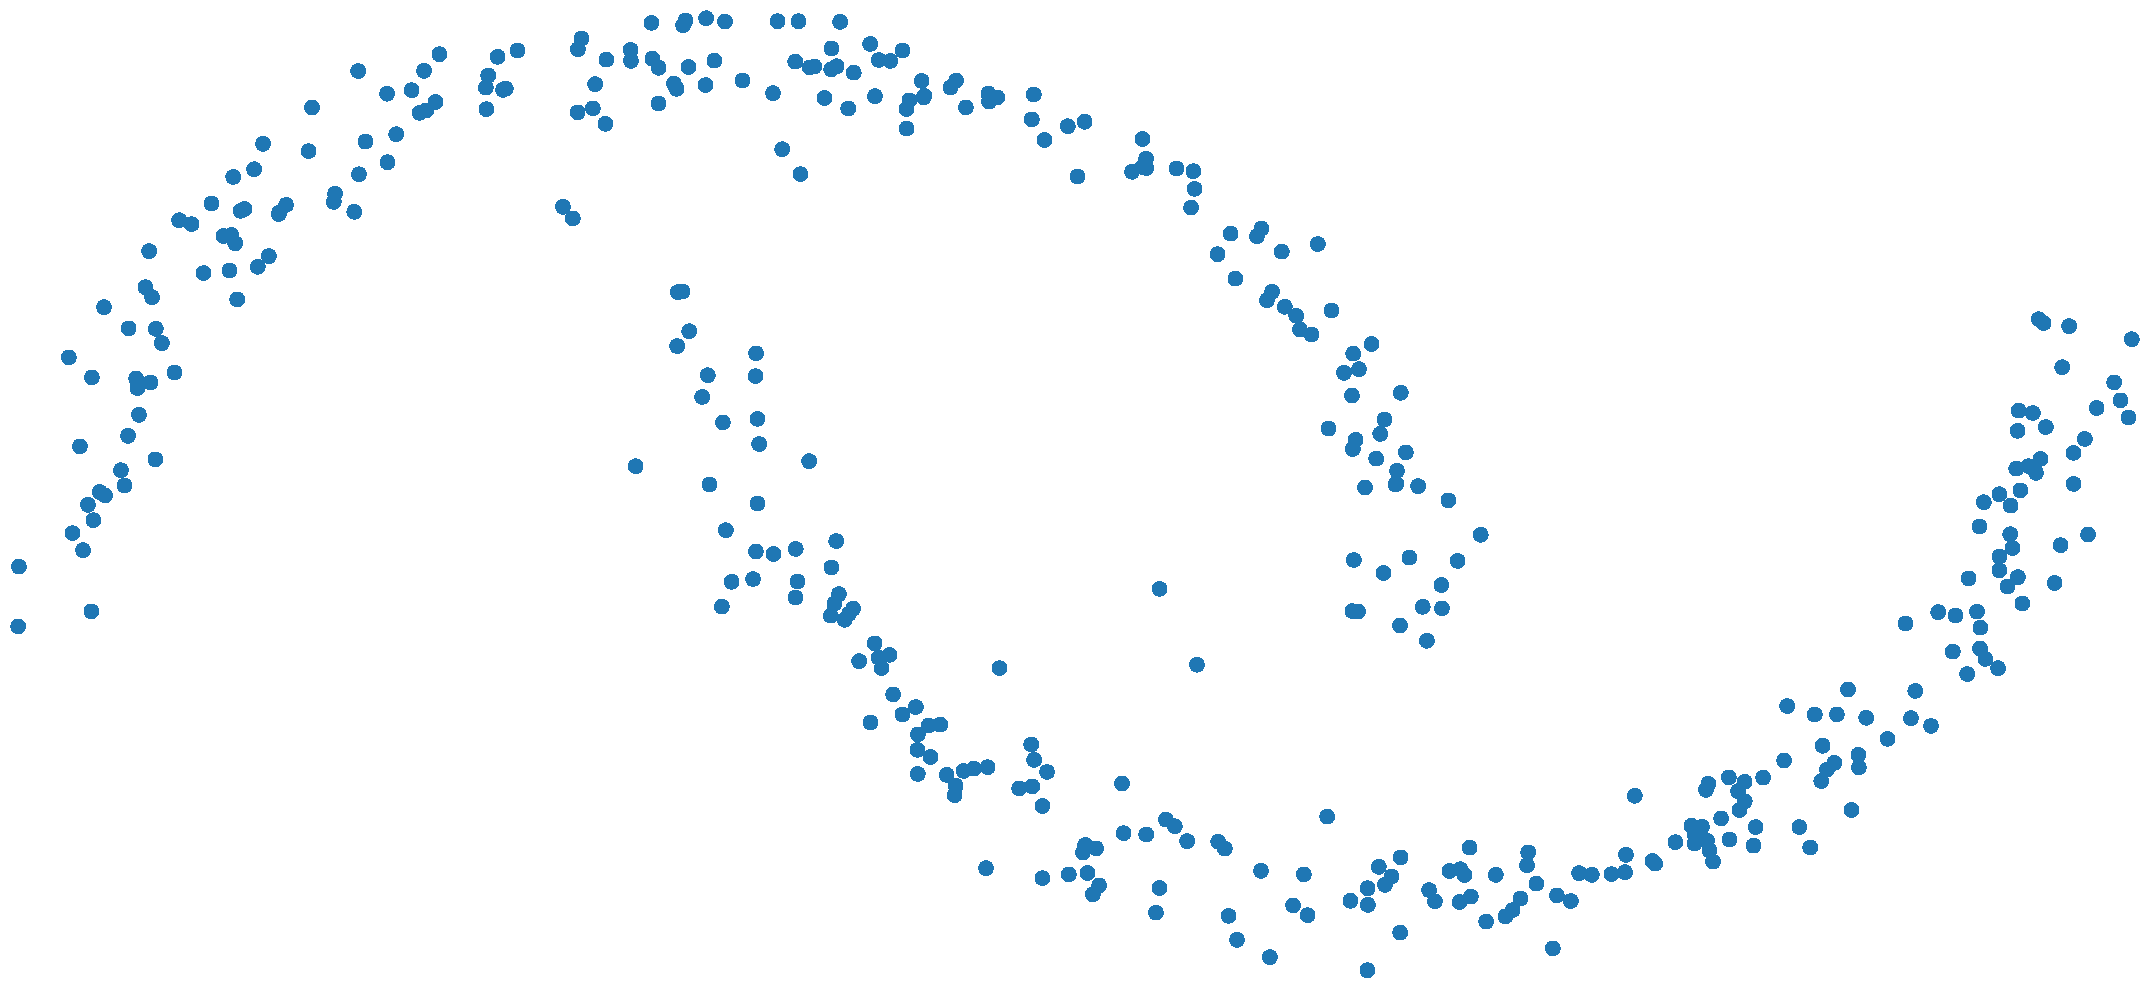
\includegraphics[width=.3\textwidth]{images/moon/xdist-crop.pdf}};
  
\end{scope}
%%% Local Variables:
%%% mode: latex
%%% TeX-master: "../ppgm_slide"
%%% End:
